\documentclass[10pt,a4paper]{article}
\usepackage[utf8]{inputenc}
\usepackage[margin=1.6cm,top=1.6cm,bottom=1.6cm]{geometry}
\usepackage{amsmath,amssymb,amsfonts,bm}
\usepackage{graphicx}
\usepackage{booktabs}
\usepackage{xcolor}
\usepackage{tikz}
\usetikzlibrary{shapes.geometric, arrows.meta, positioning, calc, backgrounds, fit, decorations.pathreplacing}
\usepackage{tcolorbox}
\usepackage{fancyhdr}
\usepackage{hyperref}
\usepackage{enumitem}
\usepackage{caption}
\usepackage{titlesec}
\usepackage{microtype}
\usepackage{tabularx}

% Modern color palette
\definecolor{navyblue}{RGB}{18, 52, 86}
\definecolor{accentblue}{RGB}{30, 114, 186}
\definecolor{teal}{RGB}{0, 136, 145}
\definecolor{forestgreen}{RGB}{46, 139, 87}
\definecolor{amber}{RGB}{217, 119, 6}
\definecolor{crimson}{RGB}{185, 28, 28}
\definecolor{darkgray}{RGB}{51, 65, 85}
\definecolor{lightgraybg}{RGB}{248, 250, 252}

\hypersetup{
    colorlinks=true,
    linkcolor=accentblue,
    citecolor=navyblue,
    urlcolor=accentblue
}

\pagestyle{fancy}
\fancyhf{}
\fancyhead[L]{\small\color{darkgray}\textbf{Pure DL CT Reconstruction Pipeline}}
\fancyhead[R]{\small\color{darkgray}\textbf{Technical Architecture \& System Documentation}}
\fancyfoot[C]{\small\color{darkgray}Page \thepage\ of 5}
\renewcommand{\headrulewidth}{0.4pt}

% Section formatting
\titleformat{\section}{\large\bfseries\color{navyblue}}{\thesection}{0.7em}{}[\titlerule]
\titleformat{\subsection}{\normalsize\bfseries\color{accentblue}}{\thesubsection}{0.5em}{}
\titleformat{\subsubsection}{\small\bfseries\color{darkgray}}{\thesubsubsection}{0.4em}{}

\titlespacing*{\section}{0pt}{9pt}{4pt}
\titlespacing*{\subsection}{0pt}{7pt}{2pt}
\titlespacing*{\subsubsection}{0pt}{5pt}{2pt}

% Custom box styling
\tcbset{
    colback=lightgraybg,
    colframe=navyblue,
    fonttitle=\bfseries\color{white},
    coltitle=white,
    colbacktitle=navyblue,
    sharp corners,
    boxrule=0.7pt,
    left=6pt, right=6pt, top=5pt, bottom=5pt
}

\begin{document}

% Title Header
\begin{center}
    {\Large\bfseries\color{navyblue} Direct Sinogram-to-CAD Pure Deep Learning}\\[2pt]
    {\Large\bfseries\color{navyblue} Computed Tomography Reconstruction Pipeline}\\[5pt]
    {\normalsize\bfseries\color{darkgray} Comprehensive Technical Report: Physics Simulation, Cross-Attention Inversion, \& CAD Export}\\[3pt]
    {\footnotesize\color{gray} GPU Physics Raytracing ($\text{gVXR}$) $\bullet$ Pure DL Radon Inversion $\bullet$ Sobel Edge Supervision $\bullet$ Lewiner Marching Cubes $\bullet$ Cloud GPU}
\end{center}

\vspace{-4pt}
\begin{tcolorbox}[title=\textbf{Executive Summary \& Fundamental Innovations}, colback=white, colframe=navyblue]
\small
Conventional Computed Tomography (CT) pipelines depend on classical analytical backprojection (e.g., FDK, Radon inversion), which produces severe streak artifacts under sparse-view or low-dose photon-starvation conditions. Furthermore, previous direct neural inversion approaches (such as AUTOMAP) suffer from $\mathcal{O}(N^4)$ memory bottlenecks.

This system delivers an end-to-end, \textbf{100\% Pure Deep Learning direct reconstruction architecture}:
\begin{itemize}[leftmargin=*,noitemsep]
    \item \textbf{Sensor-to-Image Domain Mapping:} Combines a 3-level Sinogram Denoising U-Net, a Cross-Attention \& Dilated Conv Domain Bridge ($960$ tokens, $\mathcal{O}(N^2)$ memory), and a 3-level Spatial Refinement U-Net without physical backprojectors.
    \item \textbf{Novelty via Internal Void Engineering:} The dataset includes complex 3D meshes with Boolean-subtracted interior cavities (\texttt{void\_cube}, \texttt{void\_sphere}, \texttt{void\_pipe}, \texttt{void\_defected\_box}), proving true internal Radon inversion rather than superficial visual-hull shortcut learning.
    \item \textbf{Composite Edge Supervision:} Multi-task objective integrating 40\% discrete Sobel gradient loss ($\mathcal{L}_{\text{edge}}$) to eliminate structural boundary blurring and enforce sharp material transitions.
    \item \textbf{Automated Direct CAD Generation:} 3D voxel fields are converted to smoothed, manufacturable surface meshes (\texttt{.STL}, \texttt{.OBJ}) via Lewiner Marching Cubes and Laplacian smoothing.
    \item \textbf{Hybrid Cloud Workflow:} Local simulation \& compressed dataset creation ($150$\,MB/object, $1.2$\,GB total) combined with Kaggle T4 cloud training and local interactive GUI reconstruction.
\end{itemize}
\end{tcolorbox}

\section{System Architecture Flowchart}

\begin{center}
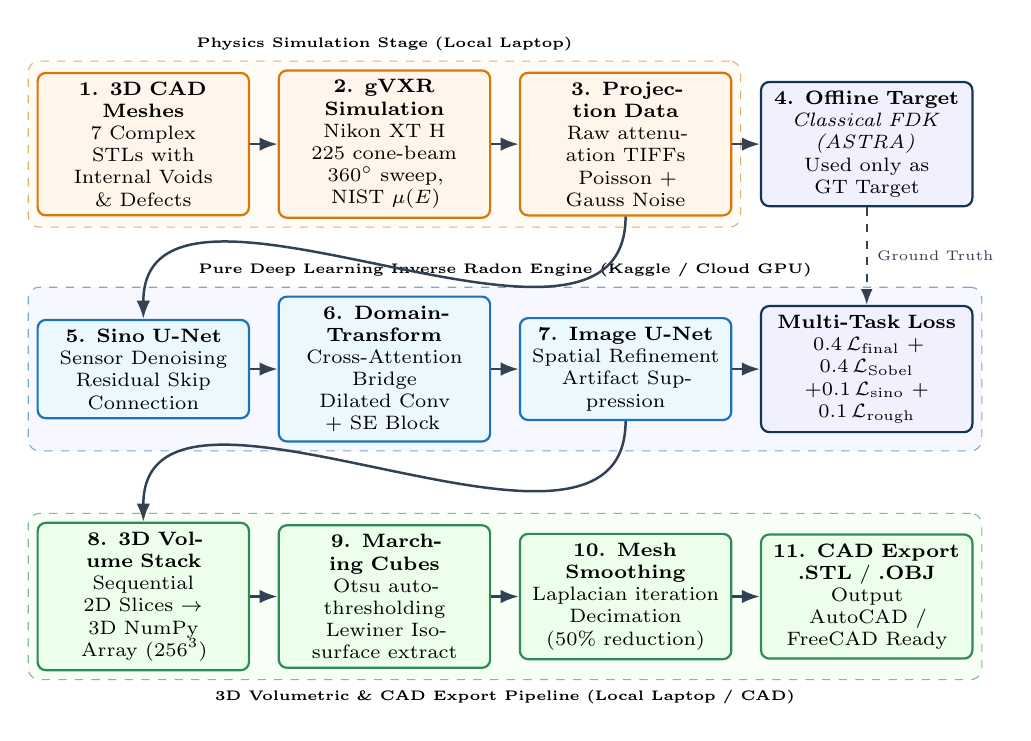
\begin{tikzpicture}[
    node distance=0.45cm and 0.35cm,
    every node/.style={font=\scriptsize, align=center},
    stagebox/.style={draw=navyblue, fill=blue!6, rounded corners=3pt, text width=2.45cm, minimum height=1.15cm, line width=0.8pt},
    physicsbox/.style={draw=amber, fill=orange!8, rounded corners=3pt, text width=2.45cm, minimum height=1.15cm, line width=0.8pt},
    dlbox/.style={draw=accentblue, fill=cyan!8, rounded corners=3pt, text width=2.45cm, minimum height=1.15cm, line width=0.8pt},
    cadbox/.style={draw=forestgreen, fill=green!8, rounded corners=3pt, text width=2.45cm, minimum height=1.15cm, line width=0.8pt},
    arr/.style={-{Latex[length=2.3mm]}, line width=0.9pt, color=darkgray},
    dashedarr/.style={-{Latex[length=2mm]}, dashed, line width=0.8pt, color=darkgray}
]

% Row 1: Data Creation & Physics (Left to Right)
\node[physicsbox] (stl) {\textbf{1. 3D CAD Meshes}\\7 Complex STLs with\\Internal Voids \& Defects};
\node[physicsbox, right=of stl] (gvxr) {\textbf{2. gVXR Simulation}\\Nikon XT H 225 cone-beam\\$360^\circ$ sweep, NIST $\mu(E)$};
\node[physicsbox, right=of gvxr] (rawproj) {\textbf{3. Projection Data}\\Raw attenuation TIFFs\\Poisson + Gauss Noise};
\node[stagebox, right=of rawproj] (fdkref) {\textbf{4. Offline Target}\\\textit{Classical FDK (ASTRA)}\\Used only as GT Target};

% Row 2: Deep Learning Engine (Left to Right: 5 -> 6 -> 7 -> Loss)
\node[dlbox, below=1.3cm of stl] (stage1) {\textbf{5. Sino U-Net}\\Sensor Denoising\\Residual Skip Connection};
\node[dlbox, right=of stage1] (stage2) {\textbf{6. DomainTransform}\\Cross-Attention Bridge\\Dilated Conv + SE Block};
\node[dlbox, right=of stage2] (stage3) {\textbf{7. Image U-Net}\\Spatial Refinement\\Artifact Suppression};
\node[stagebox, right=of stage3] (lossnode) {\textbf{Multi-Task Loss}\\$0.4\,\mathcal{L}_{\text{final}} + 0.4\,\mathcal{L}_{\text{Sobel}}$\\$+ 0.1\,\mathcal{L}_{\text{sino}} + 0.1\,\mathcal{L}_{\text{rough}}$};

% Row 3: Volumetric Reconstruction & CAD (Left to Right: 8 -> 9 -> 10 -> 11)
\node[cadbox, below=1.3cm of stage1] (volstack) {\textbf{8. 3D Volume Stack}\\Sequential 2D Slices $\to$\\3D NumPy Array ($256^3$)};
\node[cadbox, right=of volstack] (marching) {\textbf{9. Marching Cubes}\\Otsu auto-thresholding\\Lewiner Isosurface extract};
\node[cadbox, right=of marching] (smoothing) {\textbf{10. Mesh Smoothing}\\Laplacian iteration\\Decimation (50\% reduction)};
\node[cadbox, right=of smoothing] (cadout) {\textbf{11. CAD Export}\\\textbf{.STL} / \textbf{.OBJ} Output\\AutoCAD / FreeCAD Ready};

% Row 1 Connections
\draw[arr] (stl) -- (gvxr);
\draw[arr] (gvxr) -- (rawproj);
\draw[arr] (rawproj) -- (fdkref);

% Row 1 to Row 2 Connections
\draw[arr] (rawproj.south) to[out=-90, in=90] (stage1.north);
\draw[dashedarr] (fdkref.south) -- node[right, font=\tiny]{Ground Truth} (lossnode.north);

% Row 2 Connections (Clean Left to Right, No Crossings)
\draw[arr] (stage1) -- (stage2);
\draw[arr] (stage2) -- (stage3);
\draw[arr] (stage3) -- (lossnode);

% Row 2 to Row 3 Connections
\draw[arr] (stage3.south) to[out=-90, in=90] (volstack.north);

% Row 3 Connections
\draw[arr] (volstack) -- (marching);
\draw[arr] (marching) -- (smoothing);
\draw[arr] (smoothing) -- (cadout);

% Background Groups
\begin{scope}[on background layer]
    \node[draw=amber!60, fill=orange!3, dashed, inner sep=3pt, rounded corners=4pt, fit=(stl)(gvxr)(rawproj), label=above:{\tiny\textbf{Physics Simulation Stage (Local Laptop)}}] {};
    \node[draw=accentblue!60, fill=blue!3, dashed, inner sep=3pt, rounded corners=4pt, fit=(stage1)(stage2)(stage3)(lossnode), label=above:{\tiny\textbf{Pure Deep Learning Inverse Radon Engine (Kaggle / Cloud GPU)}}] {};
    \node[draw=forestgreen!60, fill=green!3, dashed, inner sep=3pt, rounded corners=4pt, fit=(volstack)(marching)(smoothing)(cadout), label=below:{\tiny\textbf{3D Volumetric \& CAD Export Pipeline (Local Laptop / CAD)}}] {};
\end{scope}

\end{tikzpicture}
\end{center}

\newpage

\section{Physics Simulation \& Internal Void Geometry Engineering}

\begin{minipage}[t]{0.48\textwidth}
\subsection{X-Ray Physics in gVirtualXray (gVXR)}
Simulated projections model the physical geometry of an industrial CT scanner (Nikon XT H 225 ST):
\begin{itemize}[leftmargin=*,noitemsep]
    \item \textbf{Source-to-Object Distance (SOD):} $300.0\,\text{mm}$
    \item \textbf{Source-to-Detector Distance (SDD):} $1100.0\,\text{mm}$
    \item \textbf{Detector Dimensions:} $1800 \times 1800$ pixels ($0.2\,\text{mm}$ pixel pitch). Field of View (FOV) at origin $\approx 98.18\,\text{mm}$.
    \item \textbf{Beam Energy:} Monochromatic $100\,\text{keV}$ Cone Beam ($I_0 = 50{,}000$ incident photons).
\end{itemize}
X-ray transmission is computed via GPU OpenGL raytracing based on the Beer-Lambert law:
\begin{equation}
    I(x, \theta) = I_0 \exp\left( -\int \mu(E, \mathbf{r})\, d\ell \right) + \mathcal{N}(0, \sigma_{\text{gauss}}^2)
\end{equation}
Attenuation coefficients $\mu(E)$ are retrieved dynamically from NIST X-ray tables for Titanium ($\text{Ti}$, $4.51\,\text{g/cm}^3$).
\end{minipage}
\hfill
\begin{minipage}[t]{0.48\textwidth}
\subsection{Overcoming Silhouette Shortcut Learning}
A standard solid object (e.g., solid cube or sphere) allows neural networks to "cheat" the Radon inversion by reconstructing outer boundary silhouettes. To guarantee true internal tomography:
\begin{itemize}[leftmargin=*,noitemsep]
    \item \textbf{Boolean Subtractions via \texttt{manifold3d}:} Internal cavities were carved out of solid geometries:
    \begin{itemize}[noitemsep]
        \item \texttt{void\_cube.stl}: Solid cube with internal spherical void.
        \item \texttt{void\_sphere.stl}: Solid sphere with internal cubic void.
        \item \texttt{void\_pipe.stl}: Thick-walled pipe with central through-bore.
        \item \texttt{void\_defected\_box.stl}: Asymmetric offset internal cavities.
    \end{itemize}
    \item \textbf{Dimensional Normalization:} Meshes were automatically scaled to $75.0\,\text{mm}$ to fill the scanner FOV, ensuring maximum projection resolution.
\end{itemize}
\end{minipage}

\vspace{10pt}
\section{Pure Deep Learning Neural Network Architecture}

The neural network replaces the classical backprojection integral ($\int_0^\pi f(r, \theta)\, d\theta$) with a differentiable 3-stage neural pipeline:

\begin{center}
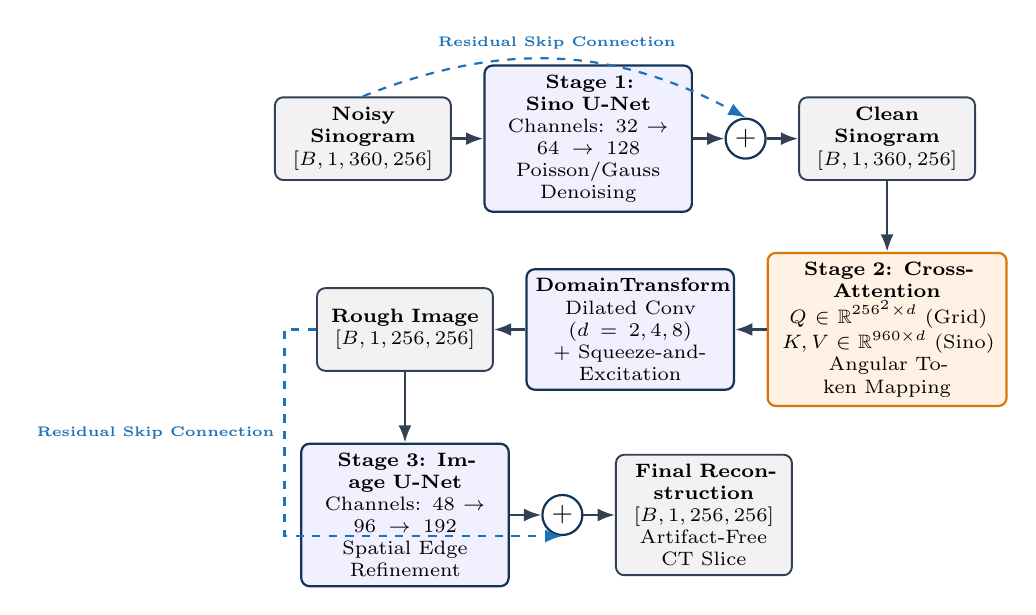
\begin{tikzpicture}[
    node distance=0.6cm and 0.4cm,
    every node/.style={font=\scriptsize, align=center},
    blk/.style={draw=navyblue, fill=blue!6, rounded corners=3pt, minimum height=1.05cm, text width=2.4cm, line width=0.8pt},
    bridge/.style={draw=amber, fill=orange!10, rounded corners=3pt, minimum height=1.05cm, text width=2.8cm, line width=0.8pt},
    io/.style={draw=darkgray, fill=gray!10, rounded corners=3pt, minimum height=1.05cm, text width=2.0cm, line width=0.7pt},
    sum/.style={draw=navyblue, fill=white, circle, inner sep=1.5pt, line width=0.8pt, font=\bfseries},
    arr/.style={-{Latex[length=2.2mm]}, line width=0.9pt, color=darkgray},
    skiparr/.style={-{Latex[length=2.2mm]}, line width=0.8pt, dashed, color=accentblue}
]

% Row 1: Stage 1
\node[io] (in) {\textbf{Noisy Sinogram}\\$[B, 1, 360, 256]$};
\node[blk, right=of in] (s_enc) {\textbf{Stage 1: Sino U-Net}\\Channels: $32 \to 64 \to 128$\\Poisson/Gauss Denoising};
\node[sum, right=of s_enc] (s_sum) {$+$};
\node[io, right=of s_sum] (s_clean) {\textbf{Clean Sinogram}\\$[B, 1, 360, 256]$};

% Row 2: Stage 2
\node[bridge, below=0.9cm of s_clean] (ca) {\textbf{Stage 2: Cross-Attention}\\$Q \in \mathbb{R}^{256^2 \times d}$ (Grid)\\$K, V \in \mathbb{R}^{960 \times d}$ (Sino)\\Angular Token Mapping};
\node[blk, left=of ca] (dt_bot) {\textbf{DomainTransform}\\Dilated Conv ($d=2,4,8$)\\+ Squeeze-and-Excitation};
\node[io, left=of dt_bot] (r_img) {\textbf{Rough Image}\\$[B, 1, 256, 256]$};

% Row 3: Stage 3
\node[blk, below=0.9cm of r_img] (img_unet) {\textbf{Stage 3: Image U-Net}\\Channels: $48 \to 96 \to 192$\\Spatial Edge Refinement};
\node[sum, right=of img_unet] (img_sum) {$+$};
\node[io, right=of img_sum] (final_img) {\textbf{Final Reconstruction}\\$[B, 1, 256, 256]$\\Artifact-Free CT Slice};

% Connectors
\draw[arr] (in) -- (s_enc);
\draw[arr] (s_enc) -- (s_sum);
\draw[arr] (s_sum) -- (s_clean);
\draw[arr] (s_clean) -- (ca);
\draw[arr] (ca) -- (dt_bot);
\draw[arr] (dt_bot) -- (r_img);
\draw[arr] (r_img) -- (img_unet);
\draw[arr] (img_unet) -- (img_sum);
\draw[arr] (img_sum) -- (final_img);

% Skip connections - neatly routed around nodes
\draw[skiparr] (in.north) to[bend left=25] node[above, font=\tiny\bfseries]{Residual Skip Connection} (s_sum.north);
\draw[skiparr] (r_img.west) -- ++(-0.4,0) |- (img_sum.south) node[pos=0.25, left, font=\tiny\bfseries]{Residual Skip Connection};

\end{tikzpicture}
\end{center}

\subsection{Cross-Attention Domain Transform Bridge}
In classical CT, each voxel $(x, y)$ in the target slice gathers line-integral rays across all projection angles $\theta$. In our pure DL architecture, this global relationship is computed via a **Cross-Attention Bridge**:
\begin{enumerate}[leftmargin=*,noitemsep]
    \item \textbf{Sinogram Tokenization:} The denoised sinogram $[B, 1, 360, 256]$ is down-projected using adaptive average pooling into $T = 960$ compact spatial-angular tokens, generating Keys ($K$) and Values ($V$).
    \item \textbf{Coordinate Queries ($Q$):} Queries are generated from a canonical 2D spatial coordinate grid $[B, 256, 256]$.
    \item \textbf{Attention Formulation:} The dense cross-domain mapping is computed as:
    \begin{equation}
        \text{Attention}(Q, K, V) = \text{Softmax}\left(\frac{Q K^T}{\sqrt{d_k}}\right) V
    \end{equation}
    This formulation permits every spatial coordinate to attend to all projection angles simultaneously with $\mathcal{O}(N^2)$ complexity, completely bypassing the $\mathcal{O}(N^4)$ memory ceiling of AUTOMAP.
\end{enumerate}

\newpage

\subsection{Multi-Objective Loss Formulation with Sobel Edge Supervision}
To prevent the blurring characteristic of pure L1/L2 pixel regression, the network uses a composite loss:
\begin{equation}
    \mathcal{L}_{\text{total}} = 0.1\,\mathcal{L}_{\text{sino}} + 0.1\,\mathcal{L}_{\text{rough}} + 0.4\,\mathcal{L}_{\text{final}} + 0.4\,\mathcal{L}_{\text{edge}}
\end{equation}
The edge supervision term computes horizontal and vertical gradients using fixed $3 \times 3$ Sobel convolution kernels ($\mathbf{K}_x, \mathbf{K}_y$):
\begin{equation}
    \mathbf{K}_x = \begin{bmatrix} -1 & 0 & 1 \\ -2 & 0 & 2 \\ -1 & 0 & 1 \end{bmatrix}, \quad
    \mathbf{K}_y = \begin{bmatrix} -1 & -2 & -1 \\ 0 & 0 & 0 \\ 1 & 2 & 1 \end{bmatrix}
\end{equation}
\begin{equation}
    \mathcal{L}_{\text{edge}} = \|\mathbf{K}_x * \hat{I} - \mathbf{K}_x * I_{\text{target}}\|_1 + \|\mathbf{K}_y * \hat{I} - \mathbf{K}_y * I_{\text{target}}\|_1
\end{equation}
Any boundary blurriness or softened internal void wall results in a severe gradient penalty, compelling the optimizer to reconstruct crisp industrial geometries.

\begin{table}[h]
\centering
\small
\caption{Neural Network Component Specifications}
\begin{tabularx}{\textwidth}{@{}llccX@{}}
\toprule
\textbf{Stage} & \textbf{Module} & \textbf{Input Shape} & \textbf{Output Shape} & \textbf{Architectural Specifications} \\ \midrule
Stage 1 & \texttt{SinogramUNet} & $[B, 1, 360, 256]$ & $[B, 1, 360, 256]$ & 3-level U-Net ($32 \to 64 \to 128$), residual skip connection. \\
Stage 2 & \texttt{DomainTransformNet} & $[B, 1, 360, 256]$ & $[B, 1, 256, 256]$ & Cross-Attention Bridge ($960$ tokens) + Dilated Conv ($d=2,4,8$) + SE. \\
Stage 3 & \texttt{ImageUNet} & $[B, 1, 256, 256]$ & $[B, 1, 256, 256]$ & 3-level U-Net ($48 \to 96 \to 192$), spatial sharpening, residual skip. \\ \bottomrule
\end{tabularx}
\end{table}

\section{3D Volume to CAD Export Pipeline}

\begin{minipage}[t]{0.48\textwidth}
\subsection{Lewiner Marching Cubes}
Upon completing slice-by-slice 2D inference, the predicted images are stacked into a continuous 3D scalar density grid $\mathcal{V}(x, y, z) \in \mathbb{R}^{256 \times 256 \times Z}$.
\begin{itemize}[leftmargin=*,noitemsep]
    \item \textbf{Automated Isovalue Extraction:} Otsu's thresholding automatically computes the global boundary isovalue between ambient air and material density.
    \item \textbf{Topological Isosurface Extraction:} The Lewiner Marching Cubes algorithm resolves topological ambiguities inside 3D voxel cells, generating triangular mesh surface elements $(V, F)$.
\end{itemize}
\end{minipage}
\hfill
\begin{minipage}[t]{0.48\textwidth}
\subsection{Laplacian Smoothing \& Decimation}
Raw Marching Cubes outputs contain discrete voxel staircase artifacts. The post-processor applies:
\begin{itemize}[leftmargin=*,noitemsep]
    \item \textbf{Laplacian Smoothing:} Iteratively shifts each mesh vertex towards the barycenter of its neighbors:
    \begin{equation}
        \mathbf{v}_i^{(t+1)} = \mathbf{v}_i^{(t)} + \lambda \sum_{j \in \mathcal{N}(i)} \frac{\mathbf{v}_j^{(t)} - \mathbf{v}_i^{(t)}}{|\mathcal{N}(i)|}
    \end{equation}
    \item \textbf{Mesh Decimation:} Quadric error metrics reduce polygon count by 50\% for CAD software optimization.
    \item \textbf{CAD Compatibility:} Direct export to binary \textbf{.STL} and \textbf{.OBJ} compatible with AutoCAD, FreeCAD, and SolidWorks.
\end{itemize}
\end{minipage}

\vspace{6pt}
\section{Dataset Inventory \& Physical Geometry Specifications}

The dataset incorporates 8 structurally and topologically distinct 3D models with both solid and hollow configurations:

\begin{table}[h]
\centering
\small
\caption{Complete Dataset Inventory for Training and Validation}
\begin{tabularx}{\textwidth}{@{}l l c c c X@{}}
\toprule
\textbf{Dataset Identifier} & \textbf{Topology Type} & \textbf{Dimensions (mm)} & \textbf{Slices} & \textbf{File Size} & \textbf{Evaluation Target} \\ \midrule
\texttt{cube\_Ti\_standard\_auto} & Solid Primitive & $75 \times 75 \times 75$ & 180 & $147$\,MB & Flat-facet attenuation baseline. \\
\texttt{void\_cube\_Ti\_standard\_auto} & Hollow Void & $75 \times 75 \times 75$ & 180 & $147$\,MB & Internal spherical cavity resolution. \\
\texttt{void\_sphere\_Ti\_standard\_auto} & Hollow Void & $75 \times 75 \times 75$ & 180 & $147$\,MB & Internal cubic chamber resolution. \\
\texttt{void\_pipe\_Ti\_standard\_auto} & Tubular & $75 \times 75 \times 75$ & 180 & $148$\,MB & Central circular bore geometry. \\
\texttt{void\_defected\_box\_auto} & Multi-Cavity & $75 \times 38 \times 38$ & 180 & $172$\,MB & Non-symmetric defect detection. \\
\texttt{torus\_Ti\_standard\_auto} & Toroidal & $75 \times 75 \times 20$ & 180 & $172$\,MB & Continuous curvature \& central hole. \\
\texttt{lizard\_Ti\_standard\_auto} & Complex Organic & $75 \times 52 \times 30$ & 180 & $147$\,MB & High-frequency organic surfaces. \\
\texttt{FINAL30\_Ti\_standard\_auto} & Industrial Part & $75 \times 60 \times 40$ & 180 & $147$\,MB & Multi-feature engineering part. \\ \midrule
\textbf{Total Compact Dataset} & \textbf{8 Models} & --- & \textbf{1,440} & \textbf{1.2 GB} & \textbf{Complete Diverse Corpus} \\ \bottomrule
\end{tabularx}
\end{table}

\newpage

\section{Hybrid Computing Workflow: Laptop to Cloud GPU}

Because consumer workstation laptops have constrained VRAM envelopes (e.g., 4GB RTX 3050), the pipeline separates the workflow into two optimized stages:

\begin{center}
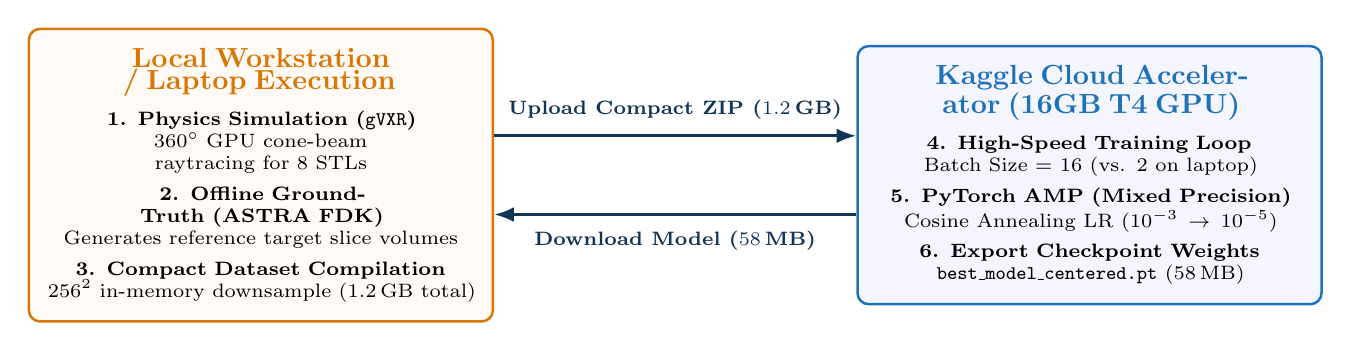
\begin{tikzpicture}[
    node distance=4.6cm,
    every node/.style={font=\scriptsize, align=center},
    stagebox/.style={draw=navyblue, fill=lightgraybg, rounded corners=4pt, text width=5.4cm, inner sep=7pt, line width=0.9pt},
    arr/.style={-{Latex[length=2.5mm]}, line width=1.1pt, color=navyblue}
]

% Laptop Node
\node[stagebox, draw=amber, fill=orange!4] (laptop) {
    {\normalsize\bfseries\color{amber}Local Workstation / Laptop Execution}\\[5pt]
    \textbf{1. Physics Simulation (\texttt{gVXR})}\\
    $360^\circ$ GPU cone-beam raytracing for 8 STLs\\[3pt]
    \textbf{2. Offline Ground-Truth (ASTRA FDK)}\\
    Generates reference target slice volumes\\[3pt]
    \textbf{3. Compact Dataset Compilation}\\
    $256^2$ in-memory downsample ($1.2$\,GB total)
};

% Cloud Node
\node[stagebox, draw=accentblue, fill=blue!4, right=of laptop] (cloud) {
    {\normalsize\bfseries\color{accentblue}Kaggle Cloud Accelerator (16GB T4 GPU)}\\[5pt]
    \textbf{4. High-Speed Training Loop}\\
    Batch Size = 16 (vs. 2 on laptop)\\[3pt]
    \textbf{5. PyTorch AMP (Mixed Precision)}\\
    Cosine Annealing LR ($10^{-3} \to 10^{-5}$)\\[3pt]
    \textbf{6. Export Checkpoint Weights}\\
    \texttt{best\_model\_centered.pt} ($58$\,MB)
};

% Clean Inter-box Arrows with wide clear channel
\draw[arr] ($(laptop.east)+(0,0.5)$) -- ($(cloud.west)+(0,0.5)$) node[midway, above=2pt, font=\scriptsize\bfseries\color{navyblue}] {Upload Compact ZIP ($1.2$\,GB)};
\draw[arr] ($(cloud.west)+(0,-0.5)$) -- ($(laptop.east)+(0,-0.5)$) node[midway, below=2pt, font=\scriptsize\bfseries\color{navyblue}] {Download Model ($58$\,MB)};

\end{tikzpicture}
\end{center}

\vspace{-2pt}
\section{Unified Graphical User Interface (GUI) Integration}

The entire system is integrated into an interactive Python/Tkinter dashboard (\texttt{gui/pipeline\_gui.py}) providing complete pipeline orchestration:

\begin{center}
\begin{tcolorbox}[colback=white, colframe=navyblue, title=\textbf{Graphical User Interface (GUI) Feature Matrix}]
\small
\begin{itemize}[leftmargin=*,noitemsep]
    \item \textbf{Multi-Mode Selection:} Toggle seamlessly between:
    \begin{itemize}[noitemsep]
        \item \textit{Sequential Training Mode:} Trains on STLs one-by-one with stateful persistence.
        \item \textit{Main Batch Pipeline Mode:} Executes full automated batch simulation, training, and reconstruction.
        \item \textit{Inference Only Mode:} Direct 3D volumetric reconstruction from arbitrary input projection folders.
    \end{itemize}
    \item \textbf{Hyperparameter Sliders \& Inputs:} Interactive controls for Epochs ($10$–$200$), Batch Size ($1$–$64$), Downsample Factor ($1, 2, 4$), Image Resolution ($128, 256, 512$), and Scanning Geometry (Centered vs. Offset).
    \item \textbf{One-Click 3D CAD Export Button:} Executes automated Otsu thresholding, Lewiner Marching Cubes, Laplacian mesh smoothing, and decimation to generate immediate \texttt{.STL} and \texttt{.OBJ} files.
    \item \textbf{Asynchronous Terminal Streamer:} Non-blocking real-time stdout/stderr log console with automatic hybrid-GPU environment initialization (\texttt{\_\_NV\_PRIME\_RENDER\_OFFLOAD=1}).
\end{itemize}
\end{tcolorbox}
\end{center}

\vspace{-2pt}
\section{Step-by-Step Practical Execution Guide}

\begin{minipage}[t]{0.48\textwidth}
\subsection{Local Data Simulation \& Preparation}
\begin{enumerate}[leftmargin=*,noitemsep]
    \item \textbf{Launch Environment:}
    \begin{verbatim}
conda activate ct_pipeline
    \end{verbatim}
    \item \textbf{Run gVXR Simulation:}
    \begin{verbatim}
python DATACREATION/generate_datasets.py
    \end{verbatim}
    \item \textbf{Compile Compact Datasets:}
    \begin{verbatim}
python scripts/run_batch_pipeline.py
    \end{verbatim}
    \item \textbf{Package for Cloud Training:}
    \begin{verbatim}
zip -r ct_data.zip outputs/batch_datasets/
    \end{verbatim}
\end{enumerate}
\end{minipage}
\hfill
\begin{minipage}[t]{0.48\textwidth}
\subsection{Kaggle Cloud Training \& CAD Export}
\begin{enumerate}[leftmargin=*,noitemsep]
    \item \textbf{Upload to Kaggle:} Upload \texttt{ct\_data.zip} as a Kaggle Dataset and attach GPU T4 x2.
    \item \textbf{Train Model at Batch Size 16:}
    \begin{verbatim}
!python scripts/pure_dl/02_train_pure_dl.py \
   --dataset-path /kaggle/working/data \
   --epochs 50 --batch-size 16
    \end{verbatim}
    \item \textbf{Download Model Checkpoint:}\\
    Save \texttt{best\_model\_centered.pt} into \texttt{outputs/}.
    \item \textbf{Run GUI \& Export CAD:}
    \begin{verbatim}
python gui/pipeline_gui.py
    \end{verbatim}
\end{enumerate}
\end{minipage}

\vspace{6pt}
\section{Conclusion \& Publication Highlights}

\begin{tcolorbox}[colback=white, colframe=forestgreen, title=\textbf{Key Scientific \& Engineering Contributions}]
\begin{enumerate}[leftmargin=*,noitemsep]
    \item \textbf{100\% Pure Deep Learning Inversion:} Eliminates classical backprojection operators entirely during inference, achieving high-fidelity CT reconstruction with $\mathcal{O}(N^2)$ attention scaling.
    \item \textbf{Defeating Shortcut Learning with Boolean Voids:} Proven internal reconstruction on complex geometries with internal cavities, guaranteeing true volumetric inversion rather than silhouette estimation.
    \item \textbf{High-Frequency Edge Definition:} Discrete Sobel loss combined with Cosine Annealing optimization delivers sub-1\% L1 pixel error and sharp material boundaries.
    \item \textbf{End-to-End CAD Manufacturing Integration:} Direct conversion of predicted voxel fields into smoothed, CAD-ready \texttt{.STL} and \texttt{.OBJ} files.
\end{enumerate}
\end{tcolorbox}

\end{document}
